\documentclass[border=10pt]{standalone}

\usepackage{tikz}
\usepackage{tikzsymbols}
\usetikzlibrary{calc,patterns,shapes.geometric}

\def\centerarc[#1](#2)(#3:#4:#5){\draw[#1] ($(#2)+({#5*cos(#3)},{#5*sin(#3)})$) arc (#3:#4:#5);}

\begin{document}
	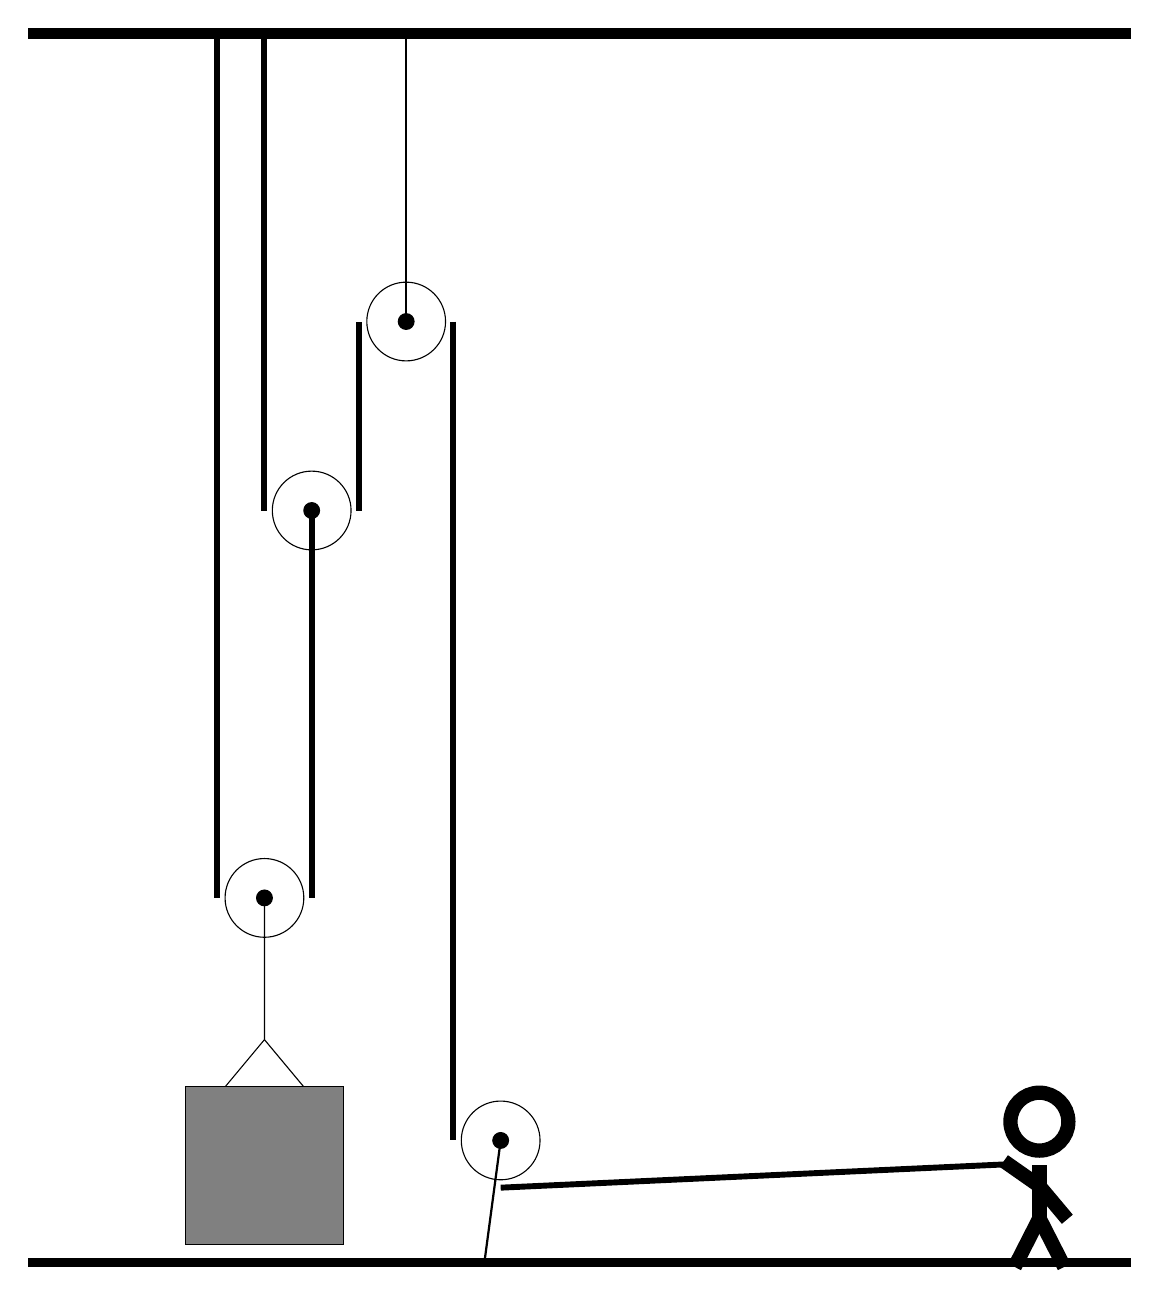
\begin{tikzpicture}
		%%%%% START %%%%%
		\draw[fill=black] (-2, 12) rectangle (12, 12.125);
		
		\draw (1, 1.08) circle (0.5);
		\draw[fill=black] (1, 1.08) circle (0.1);
		
		\draw (1.6, 6.0) circle (0.5);
		\draw[fill=black] (1.6, 6.0) circle (0.1);
		
		\draw (2.8, 8.4) circle (0.5);
		\draw[fill=black] (2.8, 8.4) circle (0.1);
		\draw[thick] (2.8, 8.4) -- (2.8, 12);
		
		\draw (4.0, -2) circle (0.5);
		\draw[fill=black] (4.0, -2) circle (0.1);
		\draw[thick] (4.0, -2) -- (3.8, -3.5);
		
		\draw (1, 1.08) -- (1, -0.72) -- (0.5, -1.32) -- (1.5, -1.32) -- (1, -0.72);
		\draw[fill=black!50] (0, -1.32) rectangle (2, -3.32);
		\draw[line width=0.75mm] (0.4, 12) -- (0.4, 1.08);
		\centerarc[line width=0.75mm](1, 1.08)(180:360:0.6);
		\draw[line width=0.75mm](1.6, 1.08) -- (1.6, 6.0);
		\draw[line width=0.75mm] (1.0, 12) -- (1.0, 6.0);
		\centerarc[line width=0.75mm](1.6, 6.0)(180:360:0.6);
		\draw[line width=0.75mm](2.2, 6.0) -- (2.2, 8.4);
		\centerarc[line width=0.75mm](2.8, 8.4)(0:180:0.6);
		\draw[line width=0.75mm] (3.4, 8.4) -- (3.4, -2);
		\centerarc[line width=0.75mm](4.0, -2)(0:90:-0.6);
		\draw[line width=0.75mm](4.0, -2.6) -- (10.5, -2.3);
		
		\node at (10.8, -2.5) {\Strichmaxerl[10][-35][-50]};
		
		\draw[fill=black] (-2, -3.5) rectangle (12, -3.6);
		%%%%% END %%%%%
	\end{tikzpicture}
\end{document}